\subsection{Product Backlog}
Para este documento, utilizamos una hoja de cálculo Excel para más comodidad y portabilidad. Primeramente se establecen las prioridades que se van a manejar dentro de los sprints para posteriormente categorizar cada historia de usuario o actividad con una de estas prioridades.
\begin{figure}[!h]
	\centering
	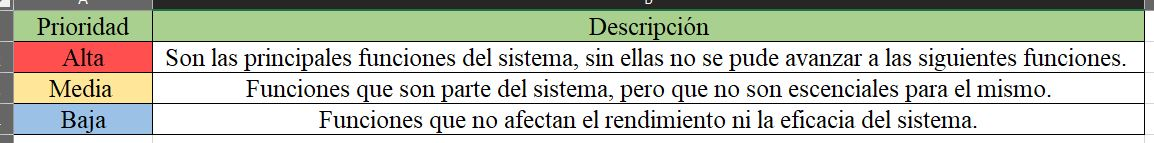
\includegraphics[width=1\textwidth]{./productBacklog/imagenes/prioridades}
	\caption{Prioridades del Product Backlog}
	\label{fig:Prioridades del Product Backlog}
\end{figure}
\subsubsection{Primer Sprint}
\begin{figure}[!h]
	\centering
	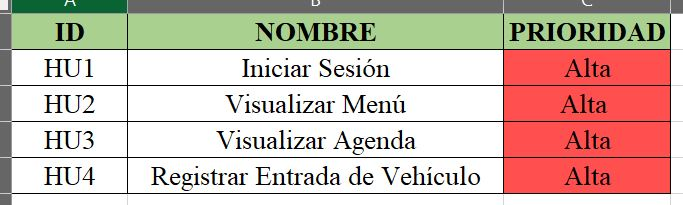
\includegraphics[width=1\textwidth]{./productBacklog/imagenes/primerSprint}
	\caption{Primer Sprint - Product Backlog}
	\label{fig:Primer Sprint - Product Backlog}
\end{figure}
\subsubsection{Segundo Sprint}
\begin{figure}[!h]
	\centering
	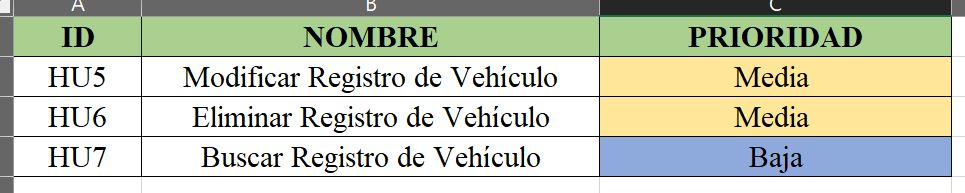
\includegraphics[width=1\textwidth]{./productBacklog/imagenes/segundoSprint}
	\caption{Segundo Sprint - Product Backlog}
	\label{fig:egundo Sprint - Product Backlog}
\end{figure}